% setup
\documentclass{beamer}
\usepackage[utf8]{inputenc}
\usepackage{graphicx}
\usetheme{Boadilla}
\usecolortheme{seahorse}

% footer 
\setbeamertemplate{footline}{
\hbox{\begin{beamercolorbox}[wd=.3\paperwidth,ht=2.25ex,dp=1ex,center]{author in head/foot}
    \usebeamerfont{author in head/foot}\insertshortauthor
  \end{beamercolorbox}%
  
  \begin{beamercolorbox}[wd=.4\paperwidth,ht=2.25ex,dp=1ex,center]{title in head/foot}%
    \usebeamerfont{title in head/foot}
    \insertsection
  \end{beamercolorbox}%
  
  \begin{beamercolorbox}[wd=.3\paperwidth,ht=2.25ex,dp=1ex,center]{author in head/foot}
    \usebeamerfont{author in head/foot}
    \insertframenumber{} / \inserttotalframenumber\hspace*{1ex}
  \end{beamercolorbox}}
}

% info for title page
\title{Semantic Image Synthesis with\newline  Spatially-Adaptive Normalization}
\subtitle{Taesung Park, Ming-Yu Liu, Ting-Chun Wang, Jun-Yan Zhu}
\author{Alexander Koenig}
\institute{Workshop in Machine Learning Applications for Computer Graphics \newline Blavatnik School of Computer Science, Tel Aviv University}
\date{April 1, 2020}

\begin{document}

% title and toc
\frame{\titlepage} 
\frame{\frametitle{Outline}\tableofcontents} 

\section{Introduction}

\begin{frame}
\frametitle{About the Paper}
\begin{itemize}
	\item published 2019
	\item by Nvidia
	\item SIGGRAPH 2019 
	\item GAN
	\item What is it for? Quick artistic sketching 
\end{itemize}

\end{frame}

\begin{frame}
\frametitle{Conditional Image Synthesis}
\begin{itemize}
	\item Conditional Image Synthesis: method to generate photorealistic images based on certain input (e.g. labels, text, ...) 
	\item Semantic Image Synthesis: method to generate photorealistic images based on semantic segmentation mask
\end{itemize}
\begin{figure}
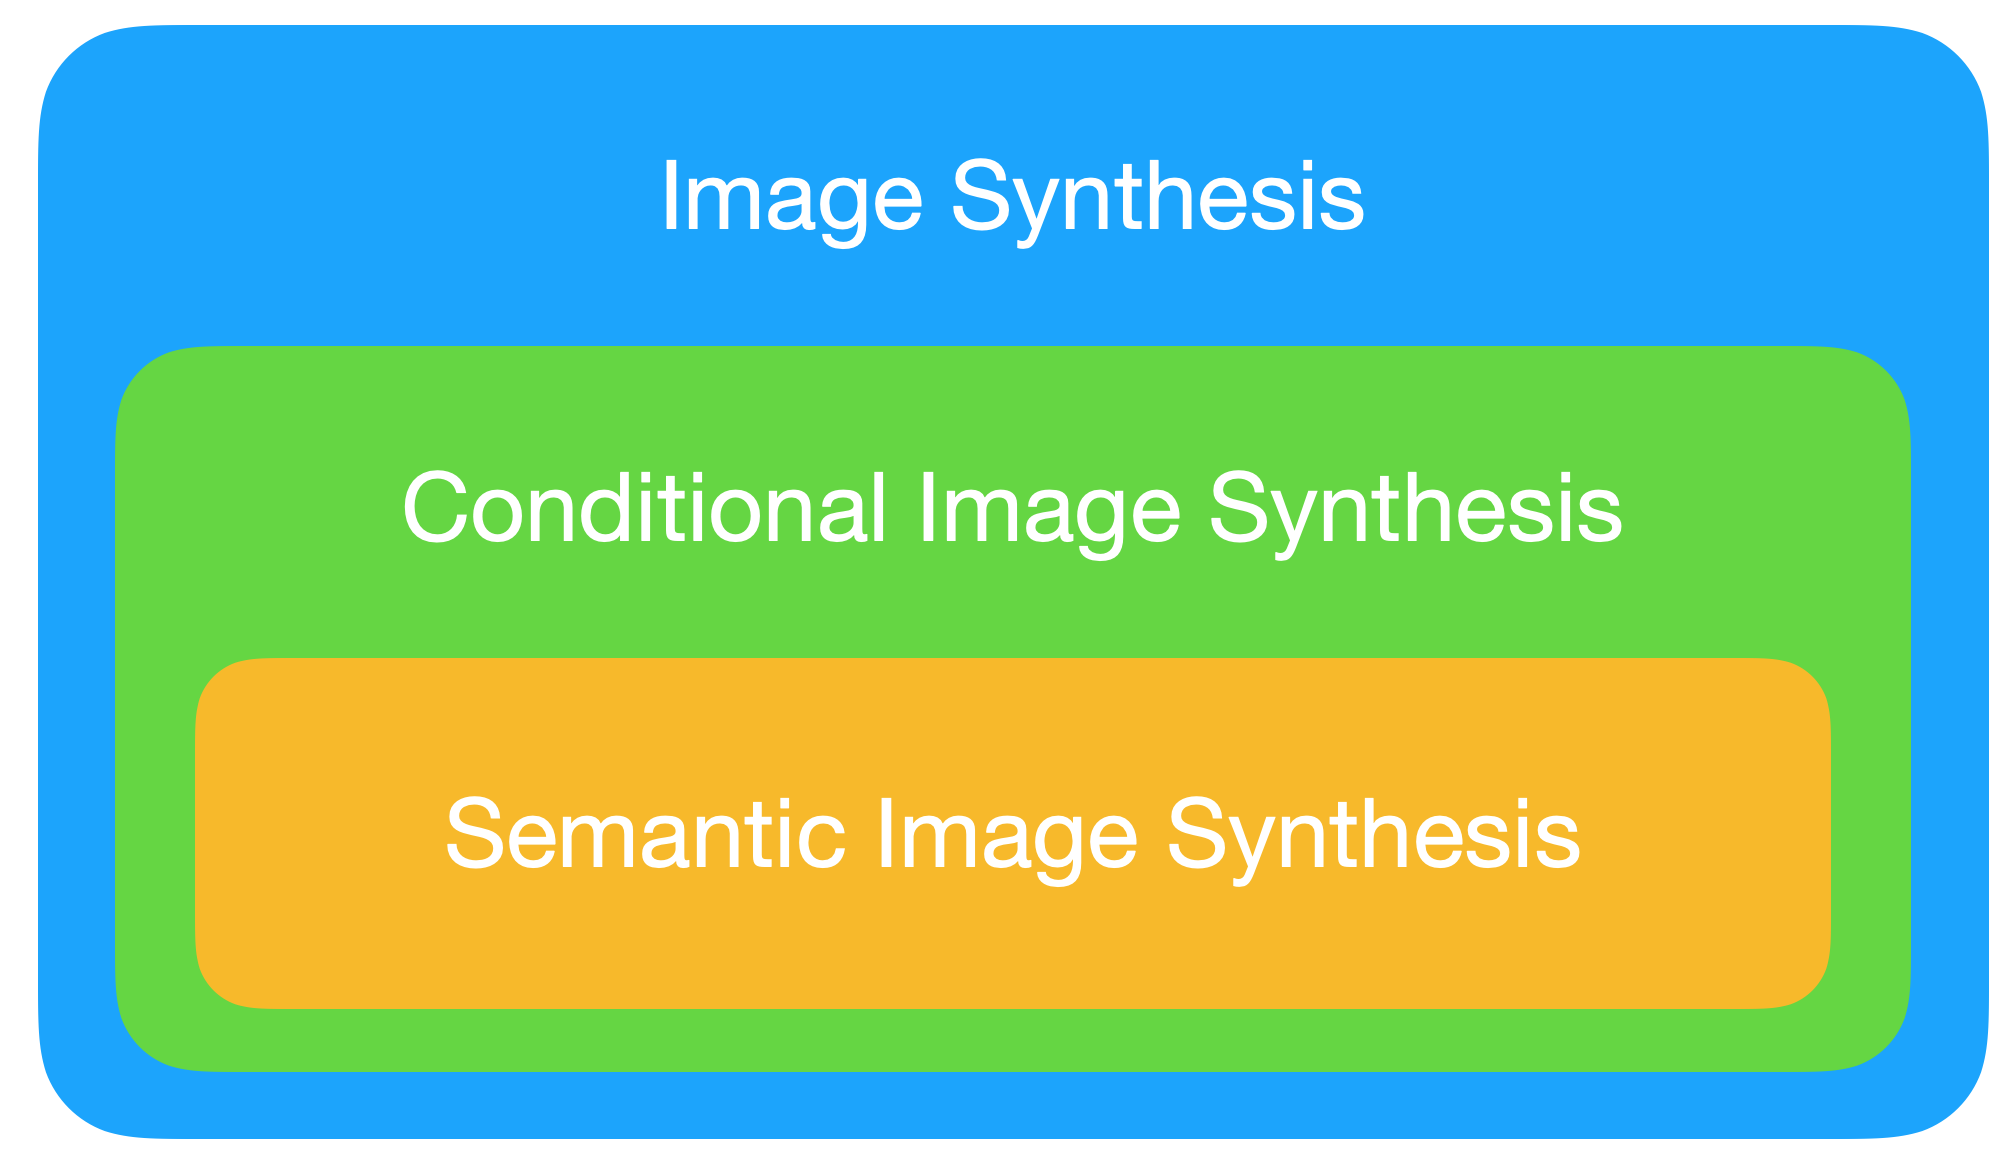
\includegraphics[scale=0.2]{figures/subsets} 
\caption{Euler diagram of image synthesis methods}
\end{figure}
\end{frame}

\section{Related Work}


\begin{frame}
	\frametitle{What is a Semantic Segmentation Mask?}
\end{frame}

\section{Semantic Image Synthesis}
\section{Experiments}
\section{Conclusion}

\end{document}